%%%%%%%%%%%%%%%%%%%%%%%%%%%%%%%%%%%%%%%%%%%%%%%%%%%%%%%%%%%%%%%%%%%%%%
%     File: ExtendedAbstract_imple.tex                               %
%     Tex Master: ExtendedAbstract.tex                               %
%                                                                    %
%     Author: Andre Calado Marta                                     %
%     Last modified : 27 Dez 2011                                    %
%%%%%%%%%%%%%%%%%%%%%%%%%%%%%%%%%%%%%%%%%%%%%%%%%%%%%%%%%%%%%%%%%%%%%%
% A Calculation section represents a practical development
% from a theoretical basis.
%%%%%%%%%%%%%%%%%%%%%%%%%%%%%%%%%%%%%%%%%%%%%%%%%%%%%%%%%%%%%%%%%%%%%%

\section{Analysis}
\label{sec:imple}

%- Granularity benchmark configurations \\
%- Signal and backgrounds \\
%- Boosted category\\
%- Experimental signature\\
%- Optimization \\
%- Event selection \\

This targets the boosted kinematic regime in which both Higgs bosons are reconstructed using large $R$ jets. The expected event topology is illustrated in figure \ref{fig:boosted}.

\begin{figure}[h]
	\centering
	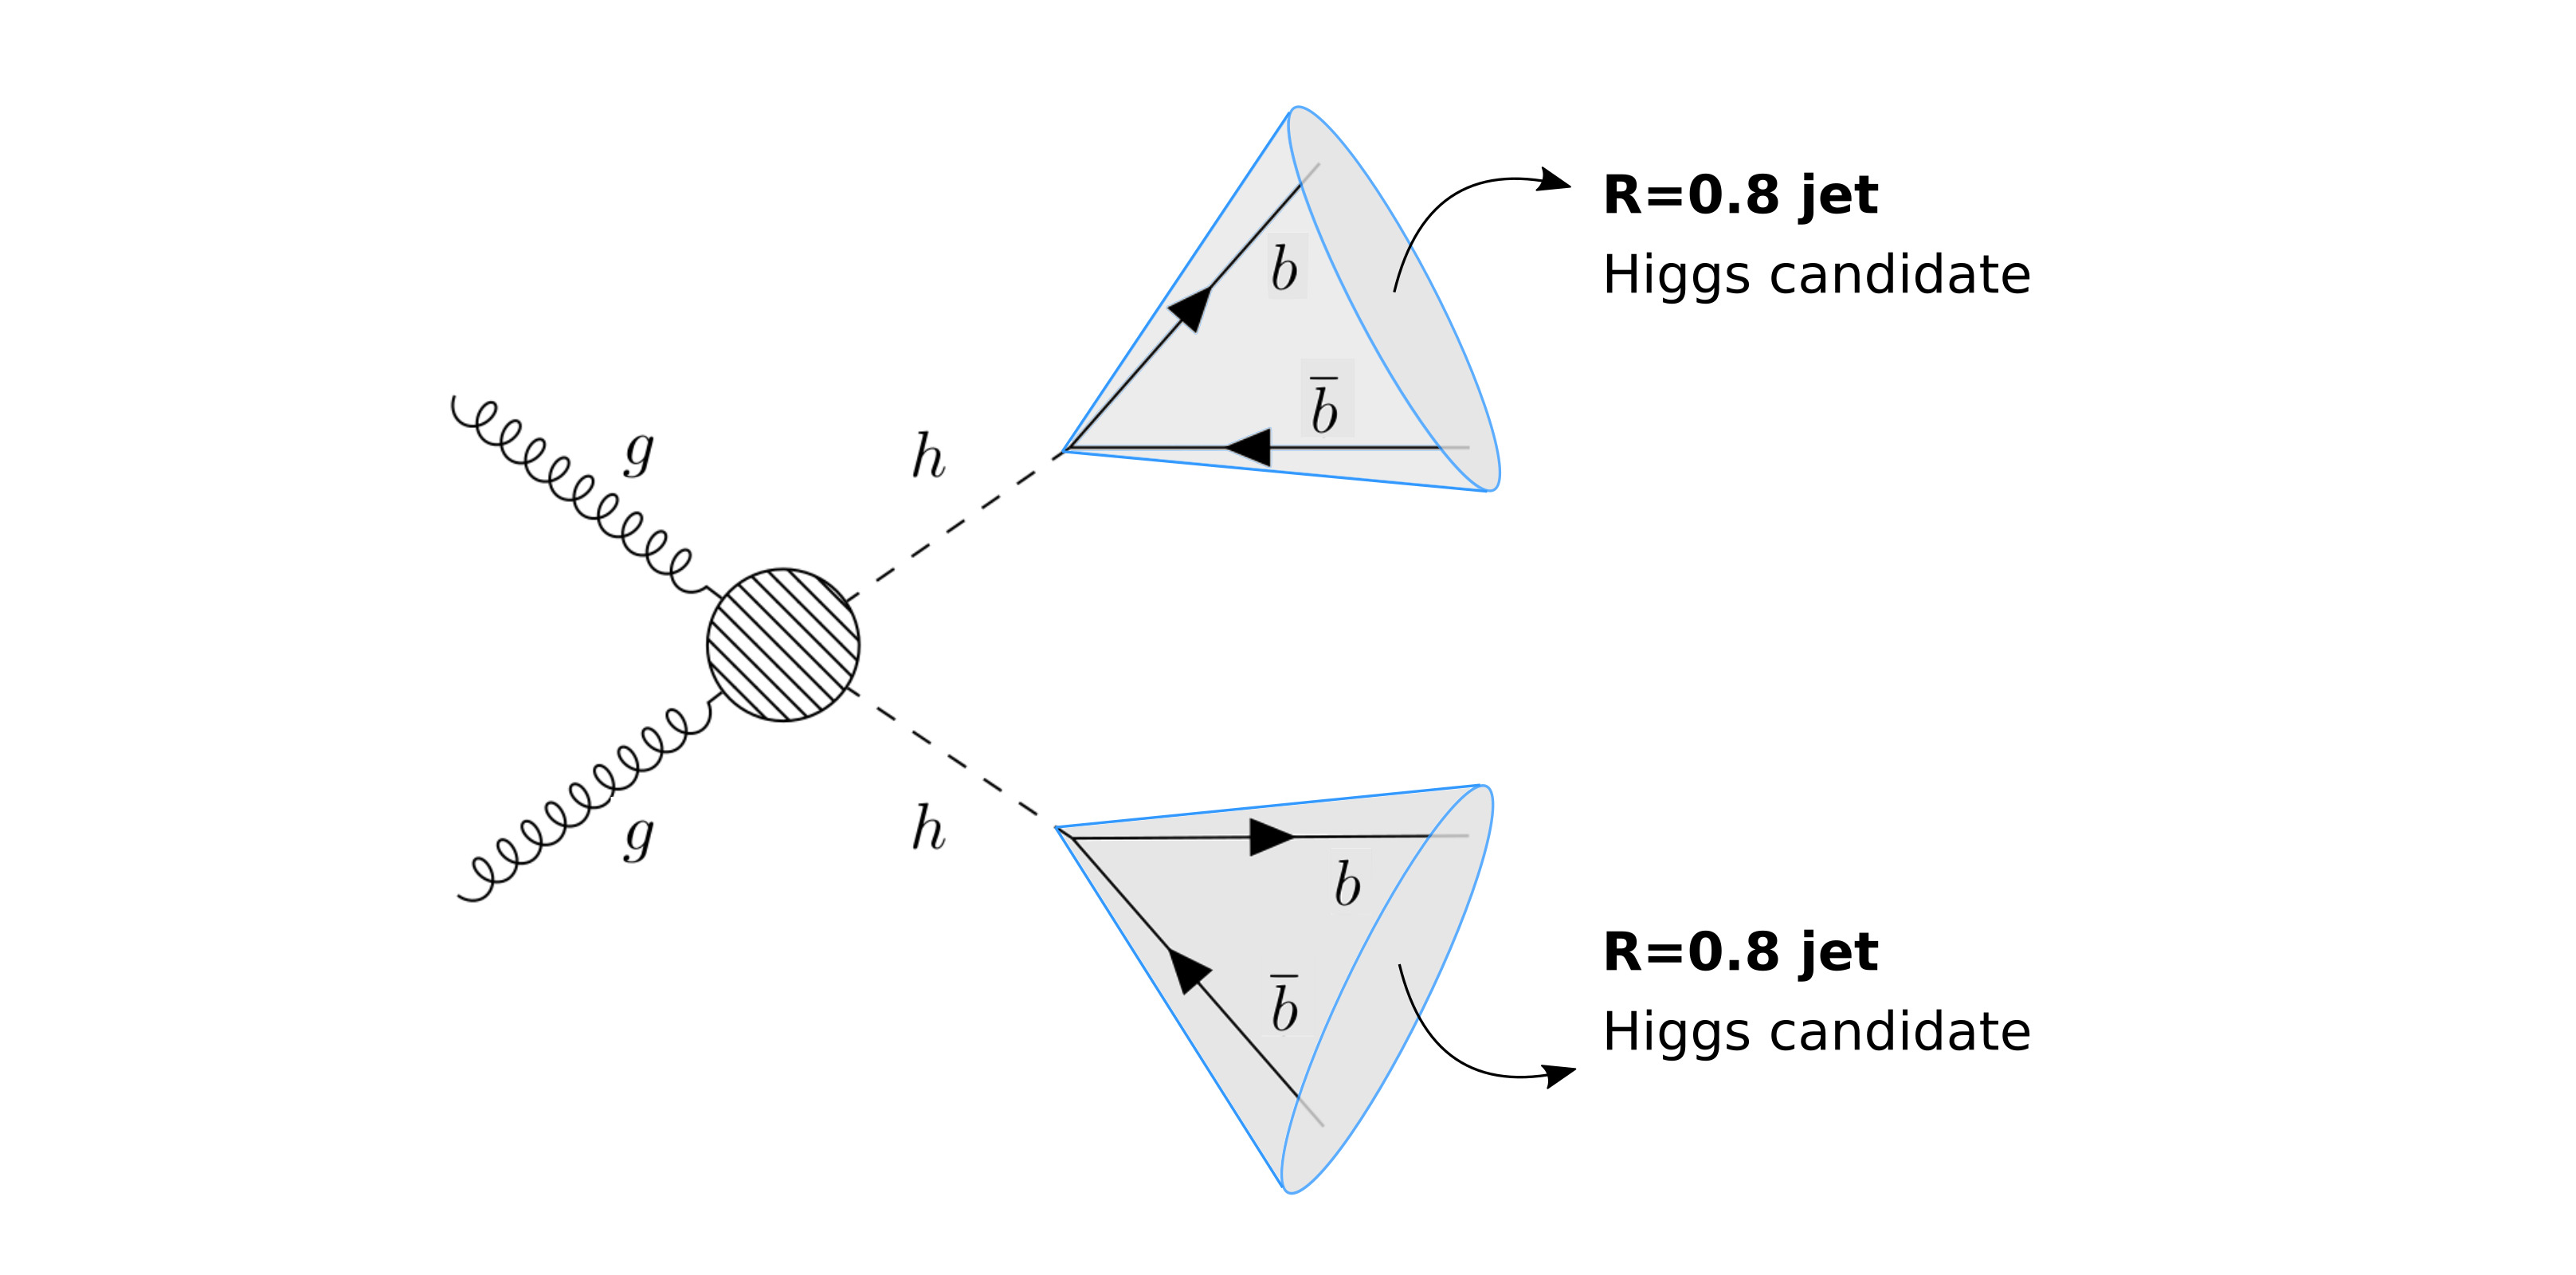
\includegraphics[trim={4.5cm .5cm 1cm .5cm},clip,width=1.2\linewidth]{./images/boosted1.png}
	\label{fig:boosted}
	\caption{oi}
\end{figure}

The events are reconstructed using particle flow (or calorimeter) jets with $R=0.8$ clustered with the anti-$k_T$ algorithm. The events are required to have at least two jets. Each jet is required to have two subjets, both b-tagged. In addition, both jets are required to have $p_T>200$ GeV. These cuts consist of the event pre-selection.

The b-tagging is implemented using truth level information. The b-tagging and mis tagging efficiencies are extracted from the FCC-hh detector default Delphes card, implemented by the FCC-hh study group.

The event selection is described in the following paragraphs. The value of the cuts follow from a scan over all the possible cut values. We choose the cut value that maximizes the significance, $S/\sqrt{B}$. 

We require
\begin{equation}
	p_T(h_1)>300~\text{GeV}, \quad p_T(hh)>100 ~\text{GeV}
\end{equation}
where $p_T(h_1)$, $p_T(hh)$ are the transverse momentums of the leading Higgs candidate and of the pair of Higgs candidates.
These cuts help suppress multijet background whose $p_T$ distributions fall more steeply than for the signal. A requirement on the maximum value of the N-subjetiness variable of the leading and subleading Higgs candidates, $\tau_{21}(h_1,h_2)]$ to further reject jets that are not consistent with a two-prong substructure:
\begin{equation}
	\tau_{21}(h_1,h_2)<0.4.
\end{equation}
These cuts work as a Higgs tagging criteria.

\begin{figure}[h]
	\centering
	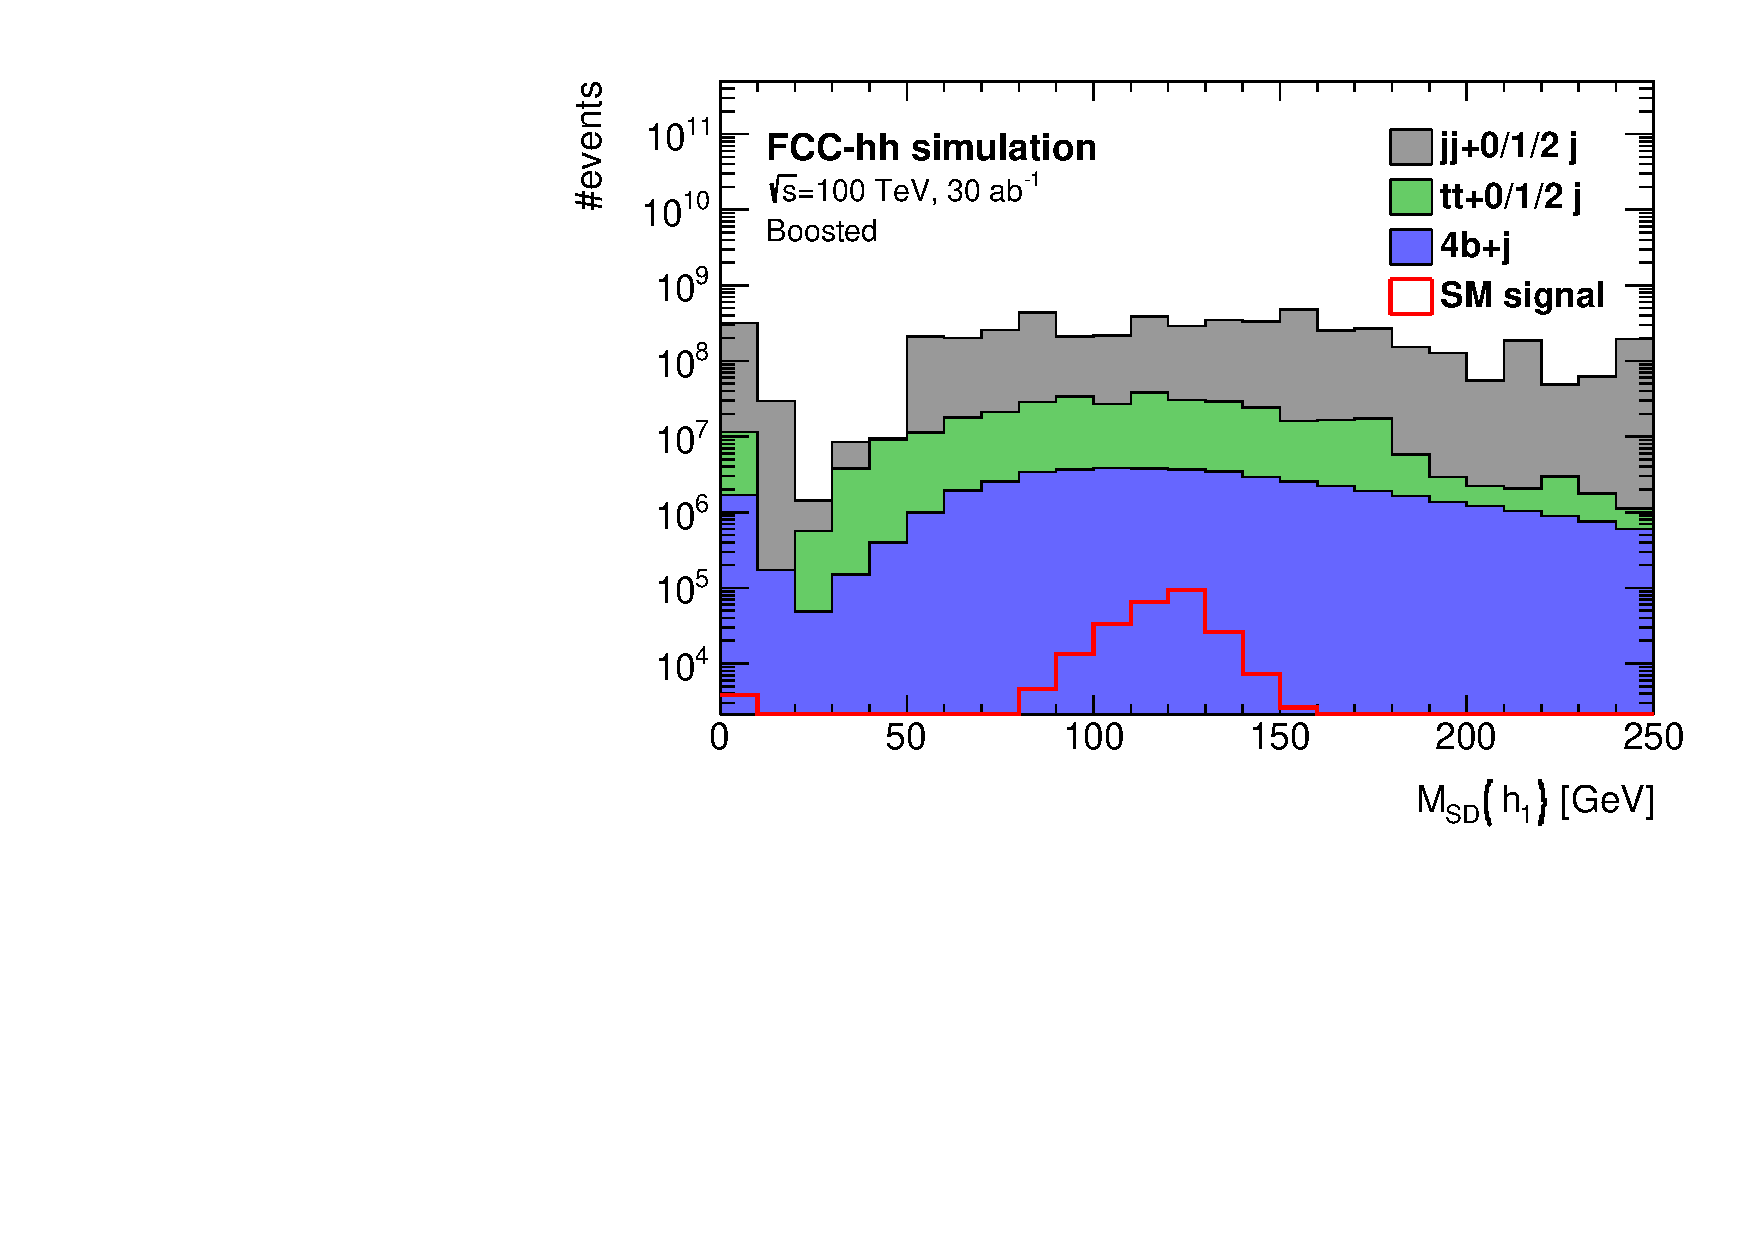
\includegraphics[width=\linewidth]{./images/hist_h1_softdrop_M_stack.pdf}
	\label{fig:stack}
	\caption{oi}
\end{figure}
